\documentclass[fsharpNotes.tex]{subfiles}
\graphicspath{ {./figures/} }

\begin{document}
\chapter{Imperative programming}
\label{cha:imperativeProgramming}
\abstract{
  Imperative programming is both and overarching term for a collection of programming paradigms and the name for specific paradigm. Here we will discuss the specific paradigm, and in \Crefrange{chap:oop}{chap:oopd} we will discuss another imperative paradigm called the object-oriented paradigm.
  % 
  When programming using the imperative paradigm, the programmer specifies a number of steps which to maninipulate the state of the computer for a desired result. Key features of this paradigm are \idx[mutable values]{mutable values} also know as \idx[variable]{variables} and \keyword{for}- and \keyword{while}-loops. In this chapter, you will learn
  \begin{itemize}
  \item How to define and use variables
  \item How to make loops using the \keyword{for}- and \keyword{while}-keywords as an alternative to recursive functions
  \item How to arrays as alternative to lists
  \item How to trace-by-hand imperative programs
  \end{itemize}
}

\section{Variables}
\label{sec:mutableValues}
A state is a value that may change over time. E.g., a traffic light as shown in \Cref{fig:trafficLight}, consists of 3 colored lamps: red (top), yellow (middle), and green (bottom), and typically cycles through the cyclic sequence red, red+yellow, green, yellow.
\begin{figure}
  \centering
  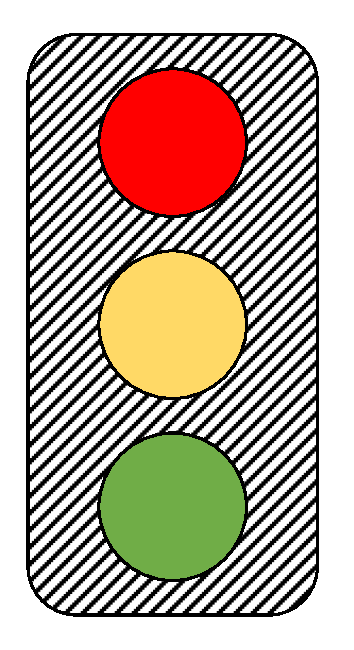
\includegraphics[width=0.3\linewidth]{trafficLight}
  \caption{For a traffic light, the different state of the coloured lamps can be modelled as different states of the ligth. Top lamp is red, middle is yellow, and bottom is green.}
  \label{fig:trafficLight}
\end{figure}
A simple model of this could be to represent the state of each lamp as being on or off. This can be done with a mutable boolean value. To create a mutable value, we initally declare and identifyer using the \idx[mutable@\lstinline{mutable}]{\keyword{mutable}} keyword with the following syntax:
%
\begin{verbatimwrite}{\ebnf/variables.ebnf}
let mutable <*ident*> = <*expr*>
\end{verbatimwrite}
\syntax{\ebnf/variables.ebnf}{Syntax for defining mutable values with an initial value.}
%
Changing the value of an identifier is called \idx{assignment} and is done using the \idx[{<-}@\lstinline{<-}]{\lexeme{<-}} lexeme. Assignments have the following syntax:\jon{Discussion on heap and stack should be added here.}
%
\begin{verbatimwrite}{\ebnf/assignment.ebnf}
<*ident*> <- <*expr*>
\end{verbatimwrite}
\syntax{\ebnf/assignment.ebnf}{Value reassignment for mutable variables.}
%
\idx[mutable value]{Mutable values} is synonymous with the term \idx{variable}. A variable is an area in the computer's working memory associated with an identifier and a type, and this area may be read from and written to during program execution, see \Cref{mutableAssignReassingShort} for an example.
%
\fs{mutableAssignReassingShort}{A variable is defined and later reassigned a new value.}
%\fs{mutableAssignReassing}{}
%
Here, an area in memory was denoted \lstinline{x}, initially assigned the integer value 5, hence the type was inferred to be \lstinline|int|.  Later, this value of \lstinline{x} was replaced with another integer using the \lexeme{<-} lexeme. The \lexeme{<-} lexeme is used to distinguish the assignment from the comparison operator. For example, the statement \lstinline{a = 3} in \Cref{mutableEqual} is not an assignment but a comparison which is evaluated to be false. 
%
\fsOutput{mutableEqual}{It is a common error to mistake \lexeme{=} and \lexeme{<-} lexemes for mutable variables.}
% \begin{lstlisting}[language=fsharp,caption={fsharpi, example of changing the content of a variable.}]
% > let mutable a = 0
% - a = 3;;
%
% val mutable a : int = 0
% val it : bool = false
% \end{lstlisting}
%
%However, it is important to note that in F\#, when the variable is initially defined, then the '\lexeme{=}' operator must be used, while later reassignments must use the \lexeme{<-} expression.

Assignment type mismatches will result in an error, as demonstrated in \Cref{mutableAssignReassingTypeError}. 
%
\fs{mutableAssignReassingTypeError}{Assignment type mismatching causes a compile-time error.}
%
I.e., once the type of an identifier has been declared or inferred, it cannot be changed.

A typical variable is a counter of type integer, and a typical use of counters is to increment them, see \Cref{mutableAssignIncrement} for an example.
%
\fs{mutableAssignIncrement}{Variable increment is a common use of variables.}
%
Using variables in expressions, as opposed to the left-hand-side of an assignment operation, reads the value of the variable. Thus, when using a variable as the return value of a function, then the value is copied from the local scope of the function to the scope from which it is called. This is demonstrated in \Cref{mutableAssignReturnVariable}.
%
\fsOutput{mutableAssignReturnVariable}{Returning a mutable variable returns its value.}
%
In the example,  we see that the type is a value, and not mutable.

In F\# it is possible to encapsulate a mutable value. For example, consider a counter function \lstinline{inc: unit->int}, which increments a counting state and returns its present value, every time we call it, i.e., calling \lstinline{inc ()} the first time should return the value 1, the second time the value 2, and so on. A first attempt could be as shown in \Cref{inc}. 
%
\fs{inc}{A failed version of the a counter function \lstinline{inc}.}
%
Even though \lstinline{inc} has an internal state, the identifier \lexeme{s} is reset to 0 every time the function is called. However, in F\# it is possible to solve this problem by using a side-effect as shown in \Cref{makeCounter}.
%
\fs{makeCounter}{Returning a counter function with a side-effect. Compare with \Cref{inc}.}
%
The reason this works is that \lstinline{makeCounter} returns a closure that includes the environment of the anonymous function at the point where it is defined. Hence, this closure includes a mutable value but does not reset it, every time it is called.


Variables implement dynamic scope, that is, the value of an identifier depends on \emph{when} it is used. This is in contrast to lexical scope, where the value of an identifier depends on \emph{where} it is defined. As an example, consider the script in \Cref{lexicalScopeNFunction} which defines a function using lexical scope and returns the number \lstinline!6.0!, however, if \lstinline!a! is made \lstinline!mutable!, then the behavior is different, as shown in \Cref{dynamicScopeNFunction}.
%
\fs{dynamicScopeNFunction}{Mutual variables implement dynamic scope rules. Compare with \Cref{lexicalScopeNFunction}.}
%
Here, the response is \lstinline!8.0!, since the value of \lstinline!a! changed before the function \lstinline!f! was called.

\section{While and For Loops}
\label{chap:flow}
This book has previously emphasized recursion as a structure to encapsulate and repeat code. In the imperative paradigm, often \idx[for@\lstinline{for}]{\keyword{for}}- and \idx[while@\lstinline{while}]{\keyword{while}}-loops are preferred. A \idx[while@\lstinline{while}]{\keyword{while}}-loop has the following syntax:
%
\begin{verbatimwrite}{\ebnf/whileLoop.ebnf}
while <*condition*> do
  <*expr*>
\end{verbatimwrite}
\syntax{\ebnf/whileLoop.ebnf}{While loop.}
%
The \idx{condition} \lstinline[language=syntax]{<*condition*>} is an expression that evaluates to true or false. A \keyword{while}-loop repeats the \lstinline[language=syntax]{<*expr*>} expression as long as the condition is true.  The \idx[do@\lstinline{do}]{\keyword{do}} keyword is mandatory and the body of the loop is indicated by indentation as usual. The return value of the \keyword{while} expression is \lexeme{()}.

The program in \Cref{count} is an example of a while-loop which counts from 1 to 10.
%
\fs{countWhile}{Count to 10 with a counter variable.}
%
Since the variable \lstinline{i} is used for counting, it is often called the counter variable. The counting is done by performing the following computation: In line~\ref{countWhileLoop}, the counter variable is first given an initial value of 1. Then in line~\ref{countWhileLoopTest}, the head of the while-loop and examines the condition. Since $1 <= 10$, the condition is true, and execution enters the body of the loop starting in line~\ref{countWhileLoopBody}. The body prints the value of the counter to the screen and increases the counter by 1. Then execution returns to the head of the while-loop and reexamines the condition. Now the condition is $2 <= 10$, which is also true, and so execution enters the body and so on until the counter has reached the value 11, in which case the condition $11 <= 10$ is false, and execution continues in line~\ref{countWhileContinue}.

Counters are so common that a special syntax has been reserved for loops using counters. These are called \idx[for-to@\lstinline{for}-\lstinline{to}]{\keyword{for}-\keyword{to}}-loops. For-loops come in several variants, and here we will focus on the one using an explicit counter. Its syntax is:
%
\begin{verbatimwrite}{\ebnf/forLoop.ebnf}
for <*ident*> = <*firstExpr*> to <*lastExpr*> do
  <*expr*>
\end{verbatimwrite}
\syntax{\ebnf/forLoop.ebnf}{For loop.}
%
A for-loop initially binds the counter identifier \lstinline[language=syntax]{<*ident*>} to be the value \lstinline[language=syntax]{<*firstExpr*>}. Then execution enters the body, and \lstinline[language=syntax]{<*bodyExpr*>} is evaluated. Once done, the counter is increased, and execution evaluates \lstinline[language=syntax]{<*bodyExpr*>}  once again. This is repeated as long as the counter is not greater than \lstinline[language=syntax]{<*lastExpr*>}. Againg, the \idx[do@\lstinline{do}]{\keyword{do}} keyword is mandatory and the body of the loop is indicated by indentation as usual. The return value of the \keyword{for} expression is \lexeme{()}.

The counting example from \Cref{countWhile} using a \keyword{for}-loop is shown in \Cref{count}
%
\fs{count}{Counting from 1 to 10 using a \keyword{for}-loop.}
%
As this interactive script demonstrates, the identifier \lstinline!i! takes all the values between 1 and 10, but in spite of its changing state, it is not mutable.

Counting backwards is sufficiently common that F\# has a \idx[for-downto@\lstinline{for}-\lstinline{downto}]{\keyword{for}-\keyword{downto}} structure, which works exactly like a \keyword{for}-\keyword{to}-loop except that the counter is decreased by 1 in each iteration. An example of this is shown in \Cref{countBackwards}.
%
\fs{countBackwards}{Counting from 10 to 1 using a \keyword{for}-\keyword{downto}-loop.}
%

There is also a customized syntax for indexing lists as shown in \Cref{listFor}
%
\fs{listFor}{Iterating over elements of a list with the \keyword{for}-\keyword{in}-loop.}
%
This particular syntax for sequentially indexing into lists using a for loop is to be prefered, since it completely avoids index-out-of-bound errors.

\section{Programming Intermezzo: Imperative Fibonacci numbers}
To further compare for- and while-loops, consider the following problem.
\begin{task}{probl:fibFor}
  Write a program that calculates the $n$'th Fibonacci number.
\end{task}
Fibonacci numbers is a sequence of numbers starting with $1, 1$, and where the next number is calculated as the sum of the previous two. Hence the first ten numbers are: $1, 1, 2, 3, 5, 8, 13, 21, 34, 55$. Fibonacci numbers are related to Golden spirals shown in \Cref{fig:goldenSpiral}.
\begin{figure}
  \centering
  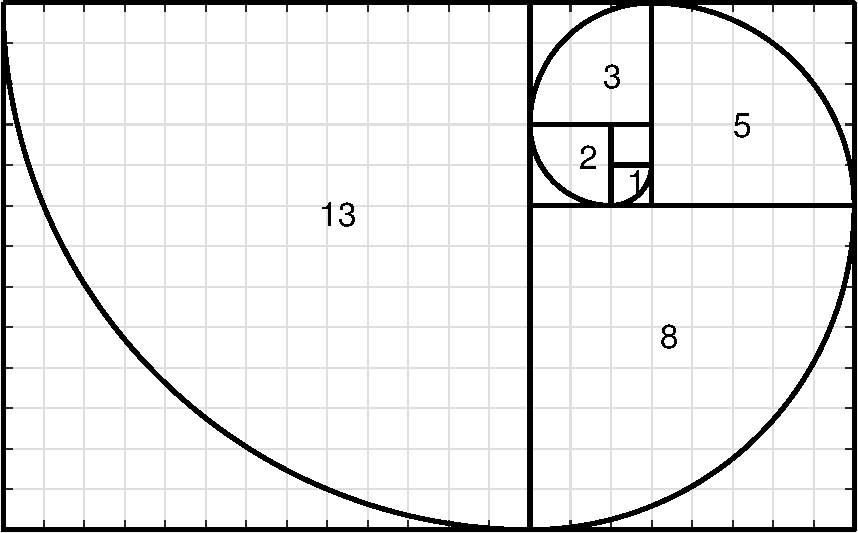
\includegraphics[width=0.45\linewidth]{Fibonacci_spiral}
  \caption{The Fibonacci spiral is an approximation of the golden spiral. Each square has side lengths of successive Fibonacci numbers, and the curve in each square is the circular arc with a radius of the square it is drawn in.}
  \label{fig:goldenSpiral}
\end{figure}
Often the sequence is extended with a preceding number $0$, to be $0, 1, 1, 2, 3, \dots$, which we will do here as well.

In \Cref{fibRecursive} we gave a solution using recursion. Here we will first use a \keyword{for}-loop, as shown in \Cref{fibFor}.
%
\fs{fibFor}{The $n$'th Fibonacci number calculated using a for-loop.}
%
The basic idea of the solution is that if we are given the $(n-1)$'th and $(n-2)$'th numbers, the $n$'th number is trivial to compute. And assuming that $\text{fib}(1)$ and $\text{fib}(2)$ are given, then it is trivial to calculate $\text{fib}(3)$. For $\text{fib}(4)$, we only need $\text{fib}(3)$ and $\text{fib}(2)$, hence we may disregard $\text{fib}(1)$. Thus, we realize that we can cyclicly update the previous, current, and next values by shifting values until we have reached the desired $\text{fib}(n)$. This is implement in \Cref{fibFor} as the function \lstinline{fib}, which takes an integer \lstinline{n} as argument and returns the $n$'th Fibonacci number. The function does this iteratively using a \keyword{for}-loop, where \lstinline{i} is the counter value, and \lstinline{pair} is the pair of the $i-1$'th and $i$'th Fibonacci numbers. In the body of the loop, the $i$'th and $i+1$'th numbers are assigned to \lstinline{pair}. The \keyword{for}-loop automatically updates \lstinline{i} for next iteration. When $n<2$ the body of the for-loop is not evaluated, and $1$ is returned. This is of course wrong for $n < 1$, but we will ignore this for now.

\Cref{fibWhile} shows a program similar to \Cref{fibFor} using a while-loop instead of for-loop.
%
\fs{fibWhile}{The $n$'th Fibonacci number calculated using a while-loop.}
%
The programs are almost identical. In this case, the \keyword{for}-loop is to be preferred, since more lines of code typically mean more chances of making a mistake.  However, while-loops are somewhat easier to argue correctness about.

\begin{comment}
The correctness of \lstinline!fib! in \Cref{fibWhile} can be proven using a \idx{loop invariant}. An \idx{invariant} is a statement that is always true at a particular point in a program, and a loop invariant is a statement which is true at the beginning and end of a loop. In line~\ref{fibWhileInvariant} in \Cref{fibWhile}, we may state the invariant: The variable \lstinline{pair} is the pair of the $i-1$'th and $i$'th Fibonacci numbers. This is provable by induction:
\begin{description}
\item[Base case:]  Before entering the while loop, \lstinline{i} is 1, \lstinline{pair} is (0, 1). Thus, the invariant is true.
\item[Induction step:] Assuming that \lstinline{pair} is the $i-1$'th and $i$'th Fibonacci numbers, the body first assigns a new value to \lstinline{pair} as the $i$'th and $i+1$'th Fibonacci numbers, then increases $i$ by one such that at the end of the loop the \lstinline{pair} again contains the the $i-1$'th and $i$'th Fibonacci numbers. \end{description}
Thus, since our invariant is true for the first case, and any iteration following an iteration where the invariant is true, is also true, then it is true for all iterations.

Thus we know that the second value in \lstinline{pair} holds the value of the $i$'th Fibonacci number, and since we further may prove that $i = n$ when line~\ref{fibWhileInvariantContinue} is reached, then it is proven that \lstinline{fib} returns the $n$'th Fibonacci number. 
\end{comment}

While-loops also allow for logical structures other than for-loops, such as the case when the number of iteration cannot easily be decided when entering the loop. As an example, consider a slight variation of the above problem, where we wish to find the largest Fibonacci number less or equal some number. A solution to this problem is shown in \Cref{fibWhileLargest}.
%
\fs{fibWhileLargest}{Search for the largest Fibonacci number less than a specified number.}
%
The strategy here is to iteratively calculate Fibonacci numbers until we've found one larger than the argument \lstinline{n}, and then return the previous. This could not be calculated with a for-loop.

\begin{comment}
  \section{Reference Cells}
\label{sec:referenceCells}
%F\# has a variation of mutable variables called \idx{reference cells}. Reference cells have built-in function \idx[ref@\lstinline{ref}]{\lstinline{ref}} and operators \idx[{!}@\lstinline{!}]{\lexeme{!}} and \idx[{:=}@\lstinline{:=}]{\lexeme{:=}}, where \lstinline{ref} creates a reference variable, and the '\lexeme{!}' and the '\lexeme{:=}' operators reads and writes its value. An example of using reference cells is given in \Cref{refCell}.
F\# has a variation of mutable variables called \idx{reference cells}. Reference cells have the built-in function \idx[ref@\lstinline{ref}]{\lstinline{ref}} and the operators \lexeme{!} and \idx[{:=}@\lstinline{:=}]{\lexeme{:=}}, where \lstinline{ref} creates a reference variable, and the '\lexeme{!}' and the '\lexeme{:=}' operators respectively reads and writes its value. An example of using reference cells is given in \Cref{refCell}.
%
\fs{refCell}{Reference cells are variants of mutable variables.}
%
Reference cells are different from mutable variables, since their content is allocated on \idx{The Heap}. The Heap is a global data storage that is not destroyed when a function returns, which is in contrast to the \idx{call stack}, also known as \idx{The Stack}. The Stack maintains all the local data for a specific instance of a function call, see \Cref{sec:callStack} for more details. As a consequence, when a reference cell is returned from a function, then it is the reference to the location on The Heap, which is returned as a value. Since this points outside the local data area of the function, this location is still valid after the function returns, and the variable stored there is accessible to the caller. This is illustrated in \Cref{fig:returningRefCells}
%
\begin{figure}
  \centering
  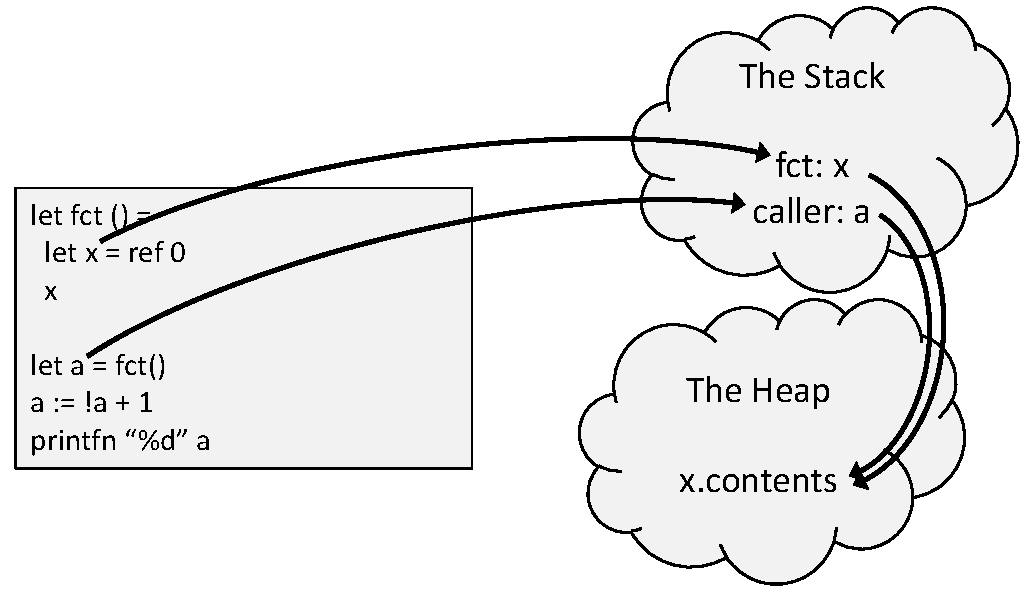
\includegraphics[width=0.6\textwidth]{ReferenceCells}
  \caption{A reference cell is a pointer to The Heap, and the content is not destroyed when its reference falls out of scope.}
  \label{fig:returningRefCells}
\end{figure}
%

Reference cells may cause \idx[side-effect]{side-effects}, where variable changes are performed across independent scopes. Some side-effects are useful, e.g., the \lstinline{printf} family changes the content of the screen, and the screen is outside the scope of the caller.  Another example of a useful side-effect is a counter shown in \Cref{refEncapsulation}.
%
\fs{refEncapsulation}{An increment function with a local state using a reference cell.}
%
Here \lstinline{incr} is an anonymous function with an internal state \lstinline{counter}. At first glance, it may be surprising that \lstinline{incr ()} does not return the value \lstinline{1} at every call. The reason is that the value of the \lstinline{incr} is the closure of the anonymous function \lstinline{fun () -> counter := ...}, which is 
\begin{equation}
  \text{\lstinline{incr}}: \left(\text{args}, \text{exp}, \text{env}\right)  = \big((), \left(\begin{subarray}{l}\displaystyle\text{\lstinline{counter := !counter + 1}}\\\displaystyle\text{\lstinline{!counter}}\end{subarray}\right), (\text{\lstinline{counter}}\rightarrow\text{\lstinline{ref 0}})\big).
\end{equation}
Thus, \lstinline{counter} is only initiated once at the initial binding, while every call of \lstinline{incr ()} updates its value on The Heap. Such a programming structure is called \idx{encapsulation}, since the \lstinline{counter} state has been encapsulated in the anonymous function, and the only way to access it is by calling the same anonymous function. In general, it is advisable to \advice{use encapsulation to hide implementation details irrelevant to the user of the code.}

The \lstinline{incr} example in \Cref{refEncapsulation} is an example of a useful side-effect. An example to be avoided is shown in \Cref{refSideEffect}.
%
\fs{refSideEffect}{Intertwining independent scopes is typically a bad idea.}
%
In the example, the function \lstinline{updateFactor} changes a variable in the scope of the function \lstinline{multiplyWithFactor}. The code style is prone to errors, since the computations are not local at the place of writing, i.e., in \lstinline{multiplyWithFactor}, and if \lstinline{updateFactor} were defined in a library, then the source code may not be available. Better style of programming is shown in \Cref{refWithoutSideEffect}.
%
\fs{refWithoutSideEffect}{A solution similar to \Cref{refSideEffect} without side-effects.}
%
Here, there can be no doubt in \lstinline{multiplyWithFactor} that the value of \lstinline{a} is changing. Side-effects do have their use, but should, in general, be avoided at almost all costs, and it is advised to \advice{minimize the use of side effects}.

Reference cells give rise to an effect called \idx{aliasing}, where two or more identifiers refer to the same data, as illustrated in \Cref{refCellAliasing}.
%
\fs{refCellAliasing}{Aliasing can cause surprising results and should be avoided.}
%
Here, \lstinline!a! is defined as a reference cell, and by defining \lstinline!b! to be equal to \lstinline!a!, we have created an alias. This can be very confusing since as the example shows, changing the value of \lstinline!b! causes \lstinline!a! to change as well. Aliasing is a variant of side-effects, and \advice{aliasing should be avoided at all costs}.

Since F\# version 4.0, the compiler has automatically converted mutable variables to reference cells, where needed.  E.g., \Cref{refEncapsulation} can be rewritten using a mutable variable, as shown in \Cref{mutableEncapsulation}.
% 
\fs{mutableEncapsulation}{Local mutable content can be indirectly accessed outside its scope.}
% 
Reference cells are preferred over mutable variables for encapsulation, in order to avoid confusion.
\end{comment}

\section{Arrays}
\label{sec:arrays}
One dimensional \idx{arrays}, or just arrays for short, are mutable lists of the same type and follow a similar syntax as lists. Arrays can be stated as a \idx{sequence expression},
%
\begin{verbatimwrite}{\ebnf/arrays.ebnf}
[|[*<*expr*>{*; <*expr*>*}*]|]
\end{verbatimwrite}
\syntax{\ebnf/arrays.ebnf}{The syntax for an array using the sequence expression.}
%
E.g., \mbox{\lstinline![|1; 2; 3|]!} is an array of integers, \mbox{\lstinline![|"This"; "is"; "an"; "array"|]!} is an array of strings, \mbox{\lstinline![|(fun x -> x); (fun x -> x*x)|]!} is an array of functions, \lstinline![||]! is the empty array.  Arrays may also be given as ranges,
%
\begin{verbatimwrite}{\ebnf/arrayRange.ebnf}
[|<*expr*> .. <*expr*> [*.. <*expr*>*]|]
\end{verbatimwrite}
\syntax{\ebnf/arrayRange.ebnf}{The syntax for an array using the range expression.}
%
but arrays of \idx{range expressions} must be of \lstinline[language=syntax]{<*expr*>} integers, floats, or characters. Examples are \mbox{\lstinline![|1 .. 5|]!}, \mbox{\lstinline![|-3.0 .. 2.0|]!}, and \mbox{\lstinline![|'a' .. 'z'|]!}. Range expressions may include a step size, thus, \mbox{\lstinline![|1 .. 2 .. 10|]!} evaluates to \mbox{\lstinline![|1; 3; 5; 7; 9|]!}.

The array type is defined using the \keyword{array} keyword or alternatively the \lexeme{[]} lexeme.  Like strings and lists, arrays may be indexed using the \idx[{[]}@\lstinline{[]}]{\lexeme{[]}} notation. Arrays cannot be resized, but are mutable, as shown in \Cref{arrayReassign}.
%
\fs{arrayReassign}{Arrays are mutable in spite of the missing \keyword{mutable} keyword.}
%
Notice that in spite of the missing \keyword{mutable} keyword, the function \lstinline{square} still has the \idx{side-effect} of squaring all entries in \lstinline{A}.  F\# implements arrays as chunks of memory and indexes arrays via address arithmetic. I.e., element $i$ in an array, whose first element is in memory address $\alpha$ and whose elements fill $\beta$ addresses each, is found at address $\alpha+i\beta$.\jon{Add a figure illustrating address indexing.} Hence, indexing has computational complexity of $\mathcal{O}(1)$, but appending and prepending values to arrays and array concatenation requires copying the new and existing values to a fresh area in memory and thus has computational complexity $\mathcal{O}(n)$, where $n$ is the total number of elements. Thus, \advice{indexing arrays is fast, but cons and concatenation is slow and should be avoided.}

Arrays support \idx{slicing}, that is, indexing an array with a range result in a copy of the array with values corresponding to the range. This is demonstrated in \Cref{arraySlicing}.
%
\fsOutput{arraySlicing}{Examples of array slicing. Compare with \Cref{listIndexing} and \Cref{stringIndexing}.}
%
As illustrated, the missing start or end index imply from the first or to the last element, respectively.

Arrays do not have explicit operator support for appending and concatenation, instead the \lstinline{Array} namespace includes an \lstinline{Array.append} function, as shown in \Cref{arrayAppend}.
%
\fs{arrayAppend}{Two arrays are appended with \lstinline{Array.append}.}
%

Arrays are \idx{reference types}, meaning that identifiers are references and thus suffer from aliasing, as illustrated in \Cref{arrayAliasing}.
%
\fs{arrayAliasing}{Arrays are reference types and suffer from aliasing.}
%
\clearpage

\subsection{Array Properties and Methods}
\label{sec:arrayMethods}
Some important properties and methods for arrays are:
\begin{description}
\item[\texttt{Clone()}:] \lstinline{'T []}.~\\
  Returns a copy of the array.
  \fsOutputNF{arrayCloneProp}{\lstinline{Clone}}\idxss{Clone@\lstinline{Clone}}
\item[\texttt{Length}:] \lstinline{int}.~\\
  Returns the number of elements in the array.
  \fsOutputNF{arrayLengthProp}{\lstinline{Length}}\idxss{Length@\lstinline{Length}}
\end{description}

\subsection{The Array Module}
\label{sec:arrayModule}
There are quite a number of built-in procedures for arrays in the \lstinline{Array} module, and many of them are almost identical to those in the \lstinline{List} module, discussed in \Cref{sec:listModule}. However, a few additional functions are noted below:
\begin{description}
\item[\texttt{Array.append}:] \lstinline{arr1:'T [] -> arr2:'T [] -> 'T []}.~\\
  Creates an new array whose elements are a concatenated copy of \lstinline{arr1} and \lstinline{arr2}.
  \fsOutputNF{arrayAppendAlt}{\lstinline{Array.append}}\idxss{Array.append@\lstinline{Array.append}}
\item[\texttt{Array.copy}:] \lstinline{'T [] -> 'T []}.~\\
  Creates an array that contains the elements of the supplied array.
  \fsOutputNF{arrayCopy}{\lstinline{Array.copy}}\idxss{Array.copy@\lstinline{Array.copy}}
\item[\texttt{Array.ofList}:] \lstinline{lst:'T list -> 'T []}.~\\
  Creates an array whose elements are copied from \lstinline{lst}.
  \fsOutputNF{arrayOflist}{\lstinline{Array.ofList}}\idxss{Array.ofList@\lstinline{Array.ofList}}
\item[\texttt{Array.toList}:] \lstinline{arr:'T [] -> 'T list}.~\\
  Creates a new list whose elements are copied from \lstinline{arr}.
  \fsOutputNF{arrayTolist}{\lstinline{Array.toList}}\idxss{Array.toList@\lstinline{Array.toList}}
\end{description}

\subsection{Multidimensional Arrays}
\idx[multidimensional arrays]{Multidimensional arrays} can be created as arrays of arrays (of arrays \dots). These are known as \idx{jagged arrays}, since there is no inherent guarantee that all sub-arrays are of the same size. The example in \Cref{arrayJagged} is a jagged array of increasing width.
%
\fs{arrayJagged}{An array of arrays of non-equal lenghts is a jagged array.}
%
Indexing arrays of arrays is done sequentially, in the sense that in the above example, the number of outer arrays is \lstinline|a.Length|,  \lstinline|a[i]| is the i'th array, the length of the i'th array is \lstinline|a[i].Length|, and the j'th element of the i'th array is thus \lstinline|a[i][j]|. Often 2-dimensional rectangular arrays are used, which can be implemented as a jagged array, as shown in \Cref{arrayJaggedSquare}.
%
\fs{arrayJaggedSquare}{A rectangular array.} 
%
Note that, the \lstinline{arr[i][j]} argument in line~\ref{arrayJaggedSquare} must be parenthesized to avoid ambiguity. Further, the \keyword{for}-\keyword{in} cannot be used in \lstinline!pownArray!, e.g., 
\begin{quote} 
  \lstinline{for row in arr do}\\
  \lstinline{  for elm in row do}\\
  \lstinline{    elm <- pown elm p}
 \end{quote}
since the iterator value \lstinline!elm! is not mutable, even though \lstinline!arr! is an array.

Square arrays of dimensions 2 to 4 are so common that F\# has built-in modules for their support. Here, we will describe \idx[Array2D@\lstinline{Array2D}]{\lstinline{Array2D}}. The workings of \idx[Array3D@\lstinline{Array3D}]{\lstinline{Array3D}} and \idx[Array4D@\lstinline{Array4D}]{\lstinline{Array4D}} are very similar. A generic \lstinline{Array2D} has type \lstinline{'T [,]}, and it is indexed also using the \lstinline|[,]| notation. The \lstinline{Array2D.length1} and \lstinline{Array2D.length2} functions are supplied by the \lstinline{Array2D} module for obtaining the size of an array along the first and second dimension. Rewriting the with jagged array example in \Cref{arrayJaggedSquare} to use \lstinline{Array2D} gives a slightly simpler program, which is shown in \Cref{array2D}.
%
\fs{array2D}{Creating a 3 by 4 rectangular array of integers.}
%
Note that the \lstinline!printf! supports direct printing of the 2-dimensional array. \lstinline{Array2D} arrays support slicing. The \lexeme{*} lexeme is particularly useful to obtain all values along a dimension. This is demonstrated in \Cref{array2DSlicing}.
%
\fsOutput{array2DSlicing}{Examples of Array2D slicing. Compare with \Cref{array2D}.}
%
Note that in almost all cases, slicing produces a sub-rectangular 2 dimensional array, except for \lstinline{arr[1,*]}, which is an array, as can be seen by the single \lexeme{[}. In contrast, \lstinline{A[1..1,*]} is an Array2D. Note also that \lstinline!printfn! typesets 2 dimensional arrays as \lstinline{[[ ... ]]} and not \lstinline{[|[| ... |]|]}, which can cause confusion with lists of lists.
%\jon{Array2D.ToString produces \lstinline{[[ ... ]]} and not \lstinline{[|[| ... |]|]}, which can cause confusion.}

Multidimensional arrays have the same properties and methods as arrays, see \Cref{sec:arrayMethods}.
\clearpage

\subsection{The Array2D Module}
The \lstinline{Array2D} module is somewhat limited. In particular neither \lstinline{fold} nor \lstinline{foldback} functions exists. Most of the module's functions are mentioned below:
\begin{description}
\item[\texttt{copy}:] \lstinline{arr:'T [,] -> 'T [,]}.~\\
  Creates a new array whose elements are copied from \lstinline{arr}.
  \fsOutputNF{array2DCopy}{\lstinline{Array2D.copy}}\idxss{Array2D.copy@\lstinline{Array2D.copy}}
\item[\texttt{create}:] \lstinline{m:int -> n:int -> v:'T -> 'T [,]}.~\\
  Creates an \lstinline{m} by \lstinline{n} array whose elements are set to \lstinline{v}.
  \fsOutputNF{array2DCreate}{\lstinline{Array2D.create}}\idxss{Array2D.create@\lstinline{Array2D.create}}
  % \item[\texttt{get}:] \lstinline{'T [,] -> int -> int -> 'T}.~\\
  %Fetches an element from a 2D array. You can also use the syntax \lstinline{array[index1,index2]}.
%  \fsOutputNF{array2DGet}{\lstinline{Array2D.get}}\idxss{Array2D.get@\lstinline{Array2D.get}}
\item[\texttt{init}:] \lstinline{m:int -> n:int -> f:(int -> int -> 'T) -> 'T [,]}.~\\
  Creates an \lstinline{m} by \lstinline{n} array whose elements are the result of applying \lstinline{f} to the index of an element.
  \fsOutputNF{array2DInit}{\lstinline{Array2D.init}}\idxss{Array2D.init@\lstinline{Array2D.init}}
\item[\texttt{iter}:] \lstinline{f:('T -> unit) -> arr:'T [,] -> unit}.~\\
  Applies \lstinline{f} to each element of \lstinline{arr}.
  \fsOutputNF{array2DIter}{\lstinline{Array2D.iter}}\idxss{Array2D.iter@\lstinline{Array2D.iter}}
\item[\texttt{length1}:] \lstinline{arr:'T [,] -> int}.~\\
  Returns the length the first dimension of \lstinline{arr}.
  \fsOutputNF{array2DLength1}{\lstinline{Array2D.length1}}\idxss{Array2D.length1@\lstinline{Array2D.length1}}
\item[\texttt{length2}:] \lstinline{arr:'T [,] -> int}.~\\
  Returns the length of the second dimension of \lstinline{arr}.
  \fsOutputNF{array2DLength2}{\lstinline{Array2D.forall length2}}\idxss{Array2D.length2@\lstinline{Array2D.length2}}
\item[\texttt{map}:] \lstinline{f:('T -> 'U) -> arr:'T [,] -> 'U [,]}.~\\
  Creates a new array whose elements are the results of applying \lstinline{f} to each of the elements of \lstinline{arr}.
  \fsOutputNF{array2DMap}{\lstinline{Array2D.map}}\idxss{Array2D.map@\lstinline{Array2D.map}}
  % \item[\texttt{set}:] \lstinline{'T [,] -> int -> int -> 'T -> unit}.~\\
  %Sets the value of an element in an array. You can also use the syntax \lstinline{array[index1,index2] <- value}.
%  \fsOutputNF{array2DSet}{\lstinline{Array2D.set}}\idxss{Array2D.set@\lstinline{Array2D.set}}
\end{description}

\begin{comment}
\section{Comparison}
% \begin{table}
%   \centering
%  \thispagestyle{empty}% empty page style (?)
  \begin{landscape}% Landscape page
    \centering % Center table
    \rowcolors{2}{oddRowColor}{evenRowColor}
    \begin{longtable}{|l|l|l|l|l|l|l|l|}
      \hline
      \rowcolor{headerRowColor} & Strings & Lists & Array & Array2D & Map & Set & Seq\\
      \hline
      {\lstinline!add : 'Key -> 'T -> Map<'Key,'T> -> Map<'Key,'T>!} & & & & & \cmark & \cmark &\\
      {\lstinline!append : 'T [] -> 'T [] -> 'T []!} & & \cmark&\cmark & & & &\cmark\\
      {\lstinline!average : 'T [] -> ^T!} & & \cmark & \cmark & & & &\cmark\\
      {\lstinline!averageBy : ('T -> ^U) -> 'T [] -> ^U!} & & \cmark & \cmark & & & &\cmark\\
      {\lstinline!base1 : 'T [,] -> int!} & & & & \cmark & & &\\
      {\lstinline!base2 : 'T [,] -> int!} & & & & \cmark & & &\\
      {\lstinline!blit : 'T [] -> int -> 'T [] -> int -> int -> unit!} & & & \cmark & \cmark & & &\\
      {\lstinline!cache : seq<'T> -> seq<'T>!} & & & & & & & \cmark\\
      {\lstinline!cast : seq<'T> -> seq<'T>!} & & & & & & & \cmark\\
      {\lstinline!choose : ('T -> 'U option) -> 'T [] -> 'U []!} & & \cmark & \cmark & & & & \cmark\\
      {\lstinline!chunkBySize : int -> 'T [] -> 'T [] []!} & & \cmark & & & & &\\
      {\lstinline!collect : ('T -> 'U []) -> 'T [] -> 'U []!} & \cmark & \cmark & \cmark & & & & \cmark\\
      {\lstinline!comparewith : ('T -> 'T -> int) -> 'T [] -> 'T [] -> int!} & & \cmark & \cmark & & & & \cmark\\
      {\lstinline!concat : seq<'T []> -> 'T []!} & \cmark & \cmark & \cmark & & & & \cmark\\
      {\lstinline!contains : 'T -> 'T [] -> bool!} & & \cmark & \cmark & & & \cmark & \cmark\\
      {\lstinline!containsKey : 'Key -> Map<'Key,'T> -> bool!} & & & & & \cmark & &\\
      {\lstinline!copy : 'T [,] -> 'T [,]!} & & & \cmark & \cmark & & &\\
      {\lstinline!count : Set<'T> -> int!} & & & & & & \cmark &\\
      {\lstinline!countBy : ('T -> 'Key) -> 'T [] -> ('Key * int) []!} & & \cmark & \cmark & & & & \cmark\\
      {\lstinline!create : int -> 'T -> 'T []!} & & & \cmark & \cmark & & &\\
      {\lstinline!createBased : int -> int -> int -> int -> 'T -> 'T [,]!} & & &  & \cmark & & &\\
      {\lstinline!delay : (unit -> seq<'T>) -> seq<'T>!} & & & & & & & \cmark\\
      {\lstinline!difference : Set<'T> -> Set<'T> -> Set<'T>!} & & & & & & \cmark &\\
      {\lstinline!distinct : 'T -> 'T []!} & & \cmark & \cmark & & & & \cmark\\
      {\lstinline!distinctBy : ('T -> 'Key) -> seq<'T> -> seq<'T>!} & & & & & & & \cmark\\
      {\lstinline!empty : 'T []!} & & \cmark & \cmark & & \cmark & \cmark & \cmark\\
      {\lstinline!exactlyOne : seq<'T> -> 'T!} & & & & & & & \cmark\\
      {\lstinline!exists : ('T -> bool) -> 'T [] -> bool!} & \cmark & \cmark & \cmark & & \cmark & \cmark & \cmark\\
      {\lstinline!exists2 : ('T1 -> 'T2 -> bool) -> 'T1 [] -> 'T2 [] -> bool!} & & \cmark & \cmark & & & & \cmark\\
      {\lstinline!fill : 'T [] -> int -> int -> 'T -> unit!} & & & \cmark & & & &\\
      {\lstinline!filter : ('T -> bool) -> 'T [] -> 'T []!} & & \cmark & \cmark & & \cmark & \cmark & \cmark\\
      {\lstinline!find : ('T -> bool) -> 'T [] -> 'T!} & & \cmark & \cmark & & \cmark & & \cmark\\
      {\lstinline!findKey : ('Key -> 'T -> bool) -> Map<'Key,'T> -> 'Key!} & & & & & \cmark & &\\
      {\lstinline!findIndex : ('T -> bool) -> 'T [] -> int!} & & \cmark & \cmark & & & & \cmark\\
      {\lstinline!fold : ('S -> 'T -> 'S) -> 'S -> 'T [] -> 'S!} & & \cmark & \cmark & & \cmark & \cmark & \cmark\\
      {\lstinline!fold2 : ('S -> 'T1 -> 'T2 -> 'S) -> 'S -> 'T1 [] -> 'T2 [] -> 'S!} & & \cmark & \cmark & & & &\\
      {\lstinline!foldBack : ('T -> 'S -> 'S) -> 'T [] -> 'S -> 'S!} & & \cmark & \cmark & & \cmark & \cmark &\\
      {\lstinline!foldBack2 : ('T1 -> 'T2 -> 'S -> 'S) -> 'T1 [] -> 'T2 [] -> 'S -> 'S!} & & \cmark & \cmark & & & &\\
      {\lstinline!forall : ('T -> bool) -> 'T [] -> bool!} & \cmark & \cmark & \cmark & & \cmark & \cmark & \cmark\\
      {\lstinline!forall2 : ('T1 -> 'T2 -> bool) -> 'T1 [] -> 'T2 [] -> bool!} & & \cmark & \cmark & & & & \cmark\\
      {\lstinline!get : 'T [] -> int -> 'T!} & & & \cmark & \cmark & & &\\
      {\lstinline!groupBy : ('T -> 'Key) -> seq<'T> -> seq<'Key * seq<'T>>!} & & & & & & & \cmark\\
      {\lstinline!head : 'T [] -> 'T!} & & \cmark &  & & & &\\
      {\lstinline!init : int -> (int -> 'T) -> 'T []!} & \cmark & \cmark & \cmark & \cmark & & & \cmark\\
      {\lstinline!initBased : int -> int -> int -> int -> (int -> int -> 'T) -> 'T [,]!} &  &  &  & \cmark & & &\\
      {\lstinline!initInfinite : (int -> 'T) -> seq<'T>!} & & & & & & & \cmark\\
      {\lstinline!intersect : Set<'T> -> Set<'T> -> Set<'T>!} & & & & & & \cmark &\\
      {\lstinline!intersectMany : seq<Set<'T>> -> Set<'T>!} & & & & & & \cmark &\\
      {\lstinline!isEmpty : 'T [] -> bool!} & & \cmark & \cmark & & \cmark & \cmark & \cmark\\
      {\lstinline!isProperSubset : Set<'T> -> Set<'T> -> bool!} & & & & & & \cmark &\\
      {\lstinline!isProperSuperset : Set<'T> -> Set<'T> -> bool!} & & & & & & \cmark &\\
      {\lstinline!isSubset : Set<'T> -> Set<'T> -> bool!} & & & & & & \cmark &\\
      {\lstinline!isSuperset : Set<'T> -> Set<'T> -> bool!} & & & & & & \cmark &\\
      {\lstinline!iter : ('T -> unit) -> 'T [] -> unit!} & \cmark & \cmark & \cmark & \cmark & \cmark & \cmark & \cmark\\
      {\lstinline!iter2 : ('T1 -> 'T2 -> unit) -> 'T1 [] -> 'T2 [] -> unit!} & & \cmark & \cmark & & & & \cmark\\
      {\lstinline!iteri : (int -> 'T -> unit) -> 'T [] -> unit!} & \cmark & \cmark & \cmark & \cmark & & & \cmark\\
      {\lstinline!iteri2 : (int -> 'T1 -> 'T2 -> unit) -> 'T1 [] -> 'T2 [] -> unit!} & & \cmark & \cmark & & & & \\
      {\lstinline!last : seq<'T> -> 'T!} & & &  & & & & \cmark\\
      {\lstinline!length : 'T [] -> int!} & \cmark & \cmark & \cmark & & & & \cmark\\
      {\lstinline!length1 : 'T [,] -> int!} & & &  & \cmark & & &\\
      {\lstinline!length2 : 'T [,] -> int!} & & &  & \cmark & & &\\
      {\lstinline!map : ('T -> 'U) -> 'T [] -> 'U []!} & \cmark & \cmark & \cmark & \cmark & \cmark & \cmark & \cmark\\
      {\lstinline!map2 : ('T1 -> 'T2 -> 'U) -> 'T1 [] -> 'T2 [] -> 'U []!} & & \cmark & \cmark & & & & \cmark\\
      {\lstinline!map3 : ('T1 -> 'T2 -> 'T3 -> 'U) -> 'T1 [] -> 'T2 [] -> 'T3 [] -> 'U []!} & & \cmark & \cmark & & & &\\
      {\lstinline!mapi : (int -> 'T -> 'U) -> 'T [] -> 'U []!} & \cmark & \cmark & \cmark & \cmark & & & \cmark\\
      {\lstinline!mapi2 : (int -> 'T1 -> 'T2 -> 'U) -> 'T1 [] -> 'T2 [] -> 'U []!} & & \cmark & \cmark & & & &\\
      {\lstinline!max : 'T [] -> 'T!} & & \cmark & \cmark & & & & \cmark\\
      {\lstinline!maxBy : ('T -> 'U) -> 'T [] -> 'T!} & & \cmark & \cmark & & & & \cmark\\
      {\lstinline!maxElement : Set<'T> -> 'T!} & & & & & & \cmark &\\
      {\lstinline!min : 'T [] -> 'T!} & & \cmark & \cmark & & & & \cmark\\
      {\lstinline!minBy : ('T -> 'U) -> 'T [] -> 'T!} & & \cmark & \cmark & & & & \cmark\\
      {\lstinline!minElement : Set<'T> -> 'T!} & & & & & & \cmark &\\
      {\lstinline!nth :  'T list -> int -> 'T!} & & & & \cmark & & & \cmark\\
      {\lstinline!rebase : 'T [,] -> 'T [,]!} & & & & \cmark & & &\\
      {\lstinline!ofArray : 'T [] -> 'T []!} & & \cmark & & & \cmark & \cmark & \cmark\\
      {\lstinline!ofList : 'T list -> 'T []!} & & & \cmark & & \cmark & \cmark & \cmark\\
      {\lstinline!ofSeq : seq<'T> -> 'T []!} & & \cmark & \cmark & \cmark & \cmark & &\\
      {\lstinline!partition : ('T -> bool) -> 'T [] * 'T []!} & & \cmark & \cmark & & \cmark & \cmark &\\
      {\lstinline!parwise : seq<'T> -> seq<'T * 'T>!} & & & & & & & \cmark\\
      {\lstinline!permute : (int -> int) -> 'T [] -> 'T []!} & & \cmark & \cmark & & & &\\
      {\lstinline!pick : ('T -> 'U option) -> 'T [] -> 'U!} & & \cmark & \cmark & & \cmark & & \cmark\\
      {\lstinline!readonly : seq<'T> -> seq<'T>!} & & & & & & & \cmark\\
      {\lstinline!reduce : ('T -> 'T -> 'T) -> 'T [] -> 'T!} & & \cmark & \cmark & & & & \cmark\\
      {\lstinline!reduceBack : ('T -> 'T -> 'T) -> 'T [] -> 'T!} & & \cmark & \cmark & & & &\\
      {\lstinline!remove : 'Key -> Map<'Key,'T> -> Map<'Key,'T>!} & & & & & \cmark & \cmark &\\
      {\lstinline!replicate : (int -> 'T -> 'T [])!} & \cmark & \cmark & \cmark & & & &\\
      {\lstinline!rev : 'T [] -> 'T []!} & & \cmark & \cmark & & & &\\
      {\lstinline!scan : ('S -> 'T -> 'S) -> 'S -> 'T [] -> 'S []!} & & \cmark & \cmark & & & & \cmark\\
      {\lstinline!scanBack : ('T -> 'S -> 'S) -> 'T [] -> 'S -> 'S []!} & & \cmark & \cmark & & & &\\
      {\lstinline!set : 'T [] -> int -> 'T -> unit!} & & & \cmark & \cmark & & &\\
      {\lstinline!singleton : 'T -> seq<'T>!} & & & & & & \cmark & \cmark\\
      {\lstinline!skip : int -> seq<'T> -> seq<'T>!} & & & & & & & \cmark\\
      {\lstinline!skipWhile : ('T -> bool) -> seq<'T> -> seq<'T>!} & & & & & & & \cmark\\
      {\lstinline!sort : 'T [] -> 'T []!} & & \cmark & \cmark & & & & \cmark\\
      {\lstinline!sortBy : ('T -> 'Key) -> 'T [] -> 'T []!} & & \cmark & \cmark & & & & \cmark\\
      {\lstinline!sortInPlace : ('T -> 'Key) -> 'T [] -> unit!} & & & \cmark & & & &\\
      {\lstinline!sortInPlaceWith : ('T -> 'T -> int) -> 'T [] -> unit!} & & & \cmark & & & &\\
      {\lstinline!sortWith : ('T -> 'T -> int) -> 'T [] -> 'T []!} & & \cmark & \cmark & & & &\\
      {\lstinline!sub : 'T [] -> int -> int -> 'T []!} & & & \cmark & & & &\\
      {\lstinline!sum : ^T [] -> ^T!} & & \cmark & \cmark & & & & \cmark\\
      {\lstinline!sumBy : ('T -> ^U) -> 'T [] -> ^U!} & & \cmark & \cmark & & & & \cmark\\
      {\lstinline!tail : 'T [] -> 'T []!} & & \cmark & & & & & \cmark\\
      {\lstinline!take : int -> seq<'T> -> seq<'T>!} & & & & & & & \cmark\\
      {\lstinline!takeWhile : ('T -> bool) -> seq<'T> -> seq<'T>'!} & & & & & & & \cmark\\
      {\lstinline!toArray : 'T list -> 'T []!} & & \cmark & & & \cmark & \cmark & \cmark\\
      {\lstinline!toList[] : 'T [] -> 'T []!} & & & \cmark & & \cmark & \cmark & \cmark\\
      {\lstinline!toSeq : 'T [] -> seq<'T>!} & & \cmark & \cmark & & \cmark & \cmark &\\
      {\lstinline!truncate : int -> seq<'T> -> seq<'T>!} & & & & & & & \cmark\\
      {\lstinline!tryFind : ('T -> bool) -> 'T [] -> 'T option!} & & \cmark & \cmark & & \cmark & & \cmark\\
      {\lstinline!tryFindIndex : ('T -> bool) -> 'T [] -> int option!} & & \cmark & \cmark & & & & \cmark\\
      {\lstinline!tryFindKey : ('Key -> 'T -> bool) -> Map<'Key,'T> -> 'Key option!} & & & & & \cmark & &\\
      {\lstinline!tryPick : ('T -> 'U option) -> 'T [] -> 'U option!} & & \cmark & \cmark & & \cmark & & \cmark\\
      {\lstinline!unfold : ('State -> 'T * 'State option) -> 'State -> seq<'T>!} & & & & & & & \cmark\\
      {\lstinline!where : ('T -> bool) -> seq<'T> -> seq<'T>!} & & & & & & & \cmark\\
      {\lstinline!windowed : int -> seq<'T> -> seq<'T []>!} & & & & & & & \cmark\\
      {\lstinline!union : Set<'T> -> Set<'T> -> Set<'T>!} & & & & & & \cmark &\\
      {\lstinline!unionMany : seq<Set<'T>> -> Set<'T>!} & & & & & & \cmark &\\
      {\lstinline!unzip : ('T1 * 'T2) [] -> 'T1 [] * 'T2 []!} & & \cmark & \cmark & & & &\\
      {\lstinline!unzip3 : ('T1 * 'T2 * 'T3) [] -> 'T1 [] * 'T2 [] * 'T3 []!} & & \cmark & \cmark & & & &\\
      {\lstinline!zeroCreate : int -> 'T []!} & & & \cmark & \cmark & & &\\
      {\lstinline!zeroCreateBased : int -> int -> int -> int-> 'T [,]!} & & & & \cmark & & &\\
      {\lstinline!zip : 'T1 [] -> 'T2 [] -> ('T1 * 'T2) []!} & & \cmark & \cmark & & & & \cmark\\
      {\lstinline!zip3 : 'T1 [] -> 'T2 [] -> 'T3 [] -> ('T1 * 'T2 * 'T3) []!} & & \cmark & \cmark & & & & \cmark\\
      \hline
    \end{longtable}
    \captionof{table}{Comparing Core.String, Collections.List, Collections.Array and Collections.Array2D, Collections.Set, Collections.Map, and Collections.Seq Modules}% Add 'table' caption
    \label{tab:listableComparision}
  \end{landscape}
%}
%  \caption{Comparing listable stuff}
%  \label{tab:listableComparision}
%\end{table}
\end{comment}    


\section{Tracing Imperative Programs}
Debugging imperative programs is more complicated than declarative programs. In particular, the notion of states require us to keep track of the dynamic scope of values. In the following, we will discuss trace-by-hand of \keyword{for}-loops followed by programs which involves states.

\subsection{Tracing Loops}
Consider the program in \Cref{printSquares}.
%
\fs{printSquares}{Print the squares of a sequence of positive integers.}
%
The program includes a function for printing the sequence of the first $N$ squares of integers. It uses a \lstinline{for}-loop with a counting value. F\# creates a new environment each time the loop body is executed. Thus, to trace this program, we mentally \idx[unfolding loops]{unfold} the loop as shown in \Cref{printSquaresUnfold}.
%
\fs{printSquaresUnfold}{An unfolded version of \Cref{printSquares}.}
%
The unfolding contains 3 new scopes lines~\ref{printSquaresUnfold:start1}--\ref{printSquaresUnfold:end1}, lines~\ref{printSquaresUnfold:start2}--\ref{printSquaresUnfold:end2}, and lines~\ref{printSquaresUnfold:start3}--\ref{printSquaresUnfold:end3}  corresponding to the 3 times, the loop is repeated, and each scope starts by binding the counting value to the name \lstinline{i}.

In the rest of this section, we will refer to the code in \Cref{printSquares}. The first rows in our tracing-table looks as follows:
\begin{quote}
  \begin{tabular*}{0.9\linewidth}{l|lll}
    Step & Line & Env.\ & Bindings and evaluations\\
    \hline
    0 & - & $E_0$ & ()\\
    1 &\ref{printSquares:N} & $E_0$ & $N = 3$\\
    2 &\ref{printSquares:squares} & $E_0$ & $\text{printSquares} = \big((n), \text{printSquares-body}, (N=3)\big)$\\
    3 &\ref{printSquares:call} & $E_0$ & $\text{printSquares } N = \text{?}$\\
  \end{tabular*}
\end{quote}
Note that due to the lexical scope rule, the closure of \lstinline{printSquares} includes \lstinline{N} in its environment element. Calling \lstinline{printSquares N} causes the creation of a new environment,
\begin{quote}
  \begin{tabular*}{0.9\linewidth}{l|lll}
    Step & Line & Env.\ & Bindings and evaluations\\
    \hline
    4 &\ref{printSquares:squares} & $E_1$ & $\big((n=3), \text{printSquares-body}, (N=3)\big)$\\
    \end{tabular*}
\end{quote}
The first statement of printSquares-body is the \lstinline{for}-loop. As our unfolding in \Cref{printSquaresUnfold} demonstrated, each time the loop-body is executed, a new scope is created with a new binding to \lstinline{i}. Reusing the notation from closures, we write
\begin{quote}
  \begin{tabular*}{0.9\linewidth}{l|lll}
    Step & Line & Env.\ & Bindings and evaluations\\
    \hline
    5 &\ref{printSquares:for} & $E_1$ & $\text{for} \dots =\text{?}$\\
  \end{tabular*}
\end{quote}
and create a new environment as if it had been a function,
\begin{quote}
  \begin{tabular*}{0.9\linewidth}{l|lll}
    Step & Line & Env.\ & Bindings and evaluations\\
    \hline
    6 &\ref{printSquares:for} & $E_2$ & $\big((i=1), \text{for-body}, (n=3,N=3)\big)$\\
    \end{tabular*}
\end{quote}
As for functions, this denotes the bindings available at beginning of the execution of the \lstinline{for}-body. The first line in the \lstinline{for}-body is the binding of the value of an expression to \lstinline{p}. The expression is \lstinline{i*i}, and to calculate its value, we look in the \lstinline{for}-loop's pseudo-closure where we find the $i=1$ binding. Hence,
\begin{quote}
  \begin{tabular*}{0.9\linewidth}{l|lll}
    Step & Line & Env.\ & Bindings and evaluations\\
    \hline
    7 &\ref{printSquares:p} & $E_2$ & $i*i = 1$\\
    8 &\ref{printSquares:p} & $E_2$ & $p = 1$\\
  \end{tabular*}
\end{quote}
The final step in the for-body is the \lstinline{printfn}-statement. Its arguments we get from the updated, active environment $E_2$ and write,
\begin{quote}
\begin{tabular*}{0.9\linewidth}{l|lll}
    Step & Line & Env.\ & Bindings and evaluations\\
    \hline
    9 &\ref{printSquares:printfn} & $E_2$ & output = ``1 : 1$\backslash$n''\\
  \end{tabular*}
\end{quote}
At this point, the \lstinline{for}-loop has reached its last line, $E_2$ is deleted, we create a new environment with the counter variable increased by 1, and repeat. Hence,
\begin{quote}
  \begin{tabular*}{0.9\linewidth}{l|lll}
    Step & Line & Env.\ & Bindings and evaluations\\
    \hline
    10 &\ref{printSquares:for} & $E_3$ & $\big((i=2), \text{for-body}, (n=3,N=3)\big)$\\
    11 &\ref{printSquares:p} & $E_3$ & $i*i = 4$\\
    12 &\ref{printSquares:p} & $E_3$ & $p = 4$\\
    13 &\ref{printSquares:printfn} & $E_3$ & output = ``2 : 4$\backslash$n''\\
  \end{tabular*}
\end{quote}
Again, we delete $E_3$, create $E_4$ where $i$ is incremented, and repeat, 
\begin{quote}
  \begin{tabular*}{0.9\linewidth}{l|lll}
    Step & Line & Env.\ & Bindings and evaluations\\
    \hline
    14 &\ref{printSquares:for} & $E_4$ & $\big((i=3), \text{for-body}, (n=3,N=3)\big)$\\
    15 &\ref{printSquares:p} & $E_4$ & $i*i = 9$\\
    16 &\ref{printSquares:p} & $E_4$ & $p = 9$\\
    17 &\ref{printSquares:printfn} & $E_4$ & output = ``3 : 9$\backslash$n''\\
  \end{tabular*}
\end{quote}
Finally, incrementing $i$ would mean that $i>n$, hence the \lstinline{for}-loop ends and as all statements returns \lstinline{()}
\begin{quote}
  \begin{tabular*}{0.9\linewidth}{l|lll}
    Step & Line & Env.\ & Bindings and evaluations\\
    \hline
    18 &\ref{printSquares:for} & $E_4$ & $\text{return} = ()$\\
  \end{tabular*}
\end{quote}
At this point, the environment $E_4$ is deleted, and we return to the enclosing environment $E_1$ and the statement or expression following Step~5. Since the \lstinline{for}-loop is the last expression in the \lstinline{printSquares} function, its return value is that of the \lstinline{for}-loop, 
\begin{quote}
  \begin{tabular*}{0.9\linewidth}{l|lll}
    Step & Line & Env.\ & Bindings and evaluations\\
    \hline
    19 &\ref{printSquares:for} & $E_1$ & $\text{return} = ()$\\
  \end{tabular*}
\end{quote}
Returning to Step~3 and environment $E_0$, we have now calculated the return-value of \lstinline{printSquares N} to be \lstinline{()}, and since this line is the last of our program, we return \lstinline{()} and end the program:
\begin{quote}
  \begin{tabular*}{0.9\linewidth}{l|lll}
    Step & Line & Env.\ & Bindings and evaluations\\
    \hline
    20 &\ref{printSquares:for} & $E_0$ & $\text{return} = ()$\\
  \end{tabular*}
\end{quote}

\subsection{Tracing Mutable Values}
For mutable bindings, the scope is dynamic. For this, we need the concept of storage. Consider the program in \Cref{dynamicScopeTracing}.
%
\fs{dynamicScopeTracing}{Example of lexical scope and closure environment.}
%
To trace the dynamic behavior of this program, we add a second table to our hand tracing, which is initially empty and has the columns Step and Value to hold the Step number when the value was updated and the value stored. For \Cref{dynamicScopeTracing}, the firsts 4 steps thus look like,
\begin{quote}
  \begin{tabular*}{0.65\linewidth}[t]{l|lll}
    Step & Line & Env.\ & Bindings and evaluations\\
    \hline
    0 & - & $E_0$ & ()\\
    1 &\ref{dynamicScopeTracing:testScope} & $E_0$ & $\text{testScope} = \big((x), \text{body}, ()\big)$\\
    2 &\ref{dynamicScopeTracing:print} & $E_0$ & $\text{testScope } 2.0 = \text{?}$\\
    3 &\ref{dynamicScopeTracing:testScope} & $E_1$ & $\big((x=2.0), \text{body}, ()\big)$\\
  \end{tabular*}
  \hspace*{0.03\linewidth}
  \begin{tabular*}{0.25\linewidth}[t]{l|l}
    Step & Value\\
    \hline
    0 & -\\
  \end{tabular*}
\end{quote}
The mutable binding in line~\ref{dynamicScopeTracing:a1} creates an internal name and a dynamic storage location. The name \lstinline{a} will be bound to a reference value, which we call $\alpha_1$, and which is a unique name shared between the two tables:
\begin{quote}
  \begin{tabular*}{0.65\linewidth}[t]{l|lll}
    Step & Line & Env.\ & Bindings and evaluations\\
    \hline
    4 &\ref{dynamicScopeTracing:a1} & $E_1$ & $a = \alpha_1$\\
  \end{tabular*}
  \hspace*{0.03\linewidth}
  \begin{tabular*}{0.25\linewidth}[t]{l|l}
    Step & Value\\
    \hline
    4 & $\alpha_1 = 3.0$\\
  \end{tabular*}
\end{quote}
The following closure of \lstinline!f! uses the reference-name instead of its value,
\begin{quote}
  \begin{tabular*}{0.65\linewidth}[t]{l|lll}
    Step & Line & Env.\ & Bindings and evaluations\\
    \hline
    5 &\ref{dynamicScopeTracing:f} & $E_1$ & $f = \big((z), a*z, (x=2.0, a=\alpha_1)\big)$\\
  \end{tabular*}
  \hspace*{0.03\linewidth}
  \begin{tabular*}{0.25\linewidth}[t]{l|l}
    Step & Value\\
    \hline
    4 & $\alpha_1 = 3.0$\\
  \end{tabular*}
\end{quote}
In line~\ref{dynamicScopeTracing:a2}, the value in the storage is updated by the assignment operator, which we denote as,
\begin{quote}
  \begin{tabular*}{0.65\linewidth}[t]{l|lll}
    Step & Line & Env.\ & Bindings and evaluations\\
    \hline
    6 &\ref{dynamicScopeTracing:a2} & $E_1$ & $a \text{ <- } 4.0$\\
  \end{tabular*}
  \hspace*{0.03\linewidth}
  \begin{tabular*}{0.25\linewidth}[t]{l|l}
    Step & Value\\
    \hline
    6 & $\alpha_1 = 4.0$\\
  \end{tabular*}
\end{quote}
Hence, when we evaluate the function \lstinline{f}, its closure looks up the value of \lstinline{a} by following the reference and finding the new value:
\begin{quote}
  \begin{tabular*}{0.65\linewidth}[t]{l|lll}
    Step & Line & Env.\ & Bindings and evaluations\\
    \hline
    7 &\ref{dynamicScopeTracing:return} & $E_1$ & $\text{f } x = \text{?}$\\
    8 &\ref{dynamicScopeTracing:return} & $E_2$ & $\big((z = 2.0), a*z, (x=2.0, a=\alpha_1)\big)$\\
    9 &\ref{dynamicScopeTracing:return} & $E_2$ & $a * z = 8.0$\\
    10 &\ref{dynamicScopeTracing:return} & $E_2$ & return = $8.0$\\
    10 &\ref{dynamicScopeTracing:return} & $E_1$ & return = $8.0$\\
    11 &\ref{dynamicScopeTracing:print} & $E_0$ & output = ``8.0$\backslash$n''\\
    12 &\ref{dynamicScopeTracing:print} & $E_0$ & $\text{return} = ()$\\
  \end{tabular*}
  \hspace*{0.03\linewidth}
  \begin{tabular*}{0.25\linewidth}[t]{l|l}
    Step & Value\\
    \hline
    6 & $\alpha_1 = 4.0$\\
  \end{tabular*}
\end{quote}
For reference, the complete pair of tables is shown in \Cref{tab:tracingDynamicScope}.
\begin{table}
  \centering
  \fbox{
    \begin{tabular*}{0.65\linewidth}[t]{l|lll}
    Step & Line & Env.\ & Bindings and evaluations\\
    \hline
    0 & - & $E_0$ & ()\\
    1 &\ref{dynamicScopeTracing:testScope} & $E_0$ & $\text{testScope} = \big((x), \text{body}, ()\big)$\\
    2 &\ref{dynamicScopeTracing:print} & $E_0$ & $\text{testScope } 2.0 = \text{?}$\\
    3 &\ref{dynamicScopeTracing:testScope} & $E_1$ & $\big((x=2.0), \text{body}, ()\big)$\\
    4 &\ref{dynamicScopeTracing:a1} & $E_1$ & $a = \alpha_1$\\
    5 &\ref{dynamicScopeTracing:f} & $E_1$ & $f = \big((z), a*z, (x=2.0, a=\alpha_1)\big)$\\
    6 &\ref{dynamicScopeTracing:a2} & $E_1$ & $a \text{ <- } 4.0$\\
    7 &\ref{dynamicScopeTracing:return} & $E_1$ & $\text{f } x = \text{?}$\\
    8 &\ref{dynamicScopeTracing:return} & $E_2$ & $\big((z = 2.0), a*z, (x=2.0, a=\alpha_1)\big)$\\
    9 &\ref{dynamicScopeTracing:return} & $E_2$ & $a * z = 8.0$\\
    10 &\ref{dynamicScopeTracing:return} & $E_2$ & return = $8.0$\\
    10 &\ref{dynamicScopeTracing:return} & $E_1$ & return = $8.0$\\
    11 &\ref{dynamicScopeTracing:print} & $E_0$ & output = ``8.0$\backslash$n''\\
    12 &\ref{dynamicScopeTracing:print} & $E_0$ & $\text{return} = ()$\\
  \end{tabular*}
  \hspace*{0.03\linewidth}
  \begin{tabular*}{0.25\linewidth}[t]{l|l}
    Step & Value\\
    \hline
    0 & -\\
    4 & $\alpha_1 = 3.0$\\
    6 & $\alpha_1 = 4.0$\\
  \end{tabular*}
  }
  \caption{The complete table produced while tracing the program in \Cref{dynamicScopeTracing} by hand.}
\label{tab:tracingDynamicScope}
\end{table}
By comparing this to the value-bindings in \Cref{lexicalScopeTracing}, we see that the mutable values give rise to a different result due to the difference between lexical and dynamic scope.

\section{Key Concepts and Terms in This Chapter}
In this chapter, we have looked at programming with states using the imperative programming paradigm. You have seen how to:
\begin{itemize}
\item define \textbf{mutable variables} and make loops with \textbf{while}- and \textbf{for}- loops
\item work with \textbf{arrays}, \textbf{jagged arrays}, and \textbf{2-dimensional arrays}.
\item \textbf{trace-by-hand} programs involving mutable values and for-loops.
\end{itemize}
\end{document}
